\section{RRTBidir\-Balanced  Class Reference}
\label{classRRTBidirBalanced}\index{RRTBidirBalanced@{RRTBidir\-Balanced}}
Balanced Bidirectional {\bf RRTCon\-Con} {\rm (p.\,\pageref{classRRTConCon})} planner. 


{\tt \#include $<$rrt.h$>$}

Inheritance diagram for RRTBidir\-Balanced::\begin{figure}[H]
\begin{center}
\leavevmode
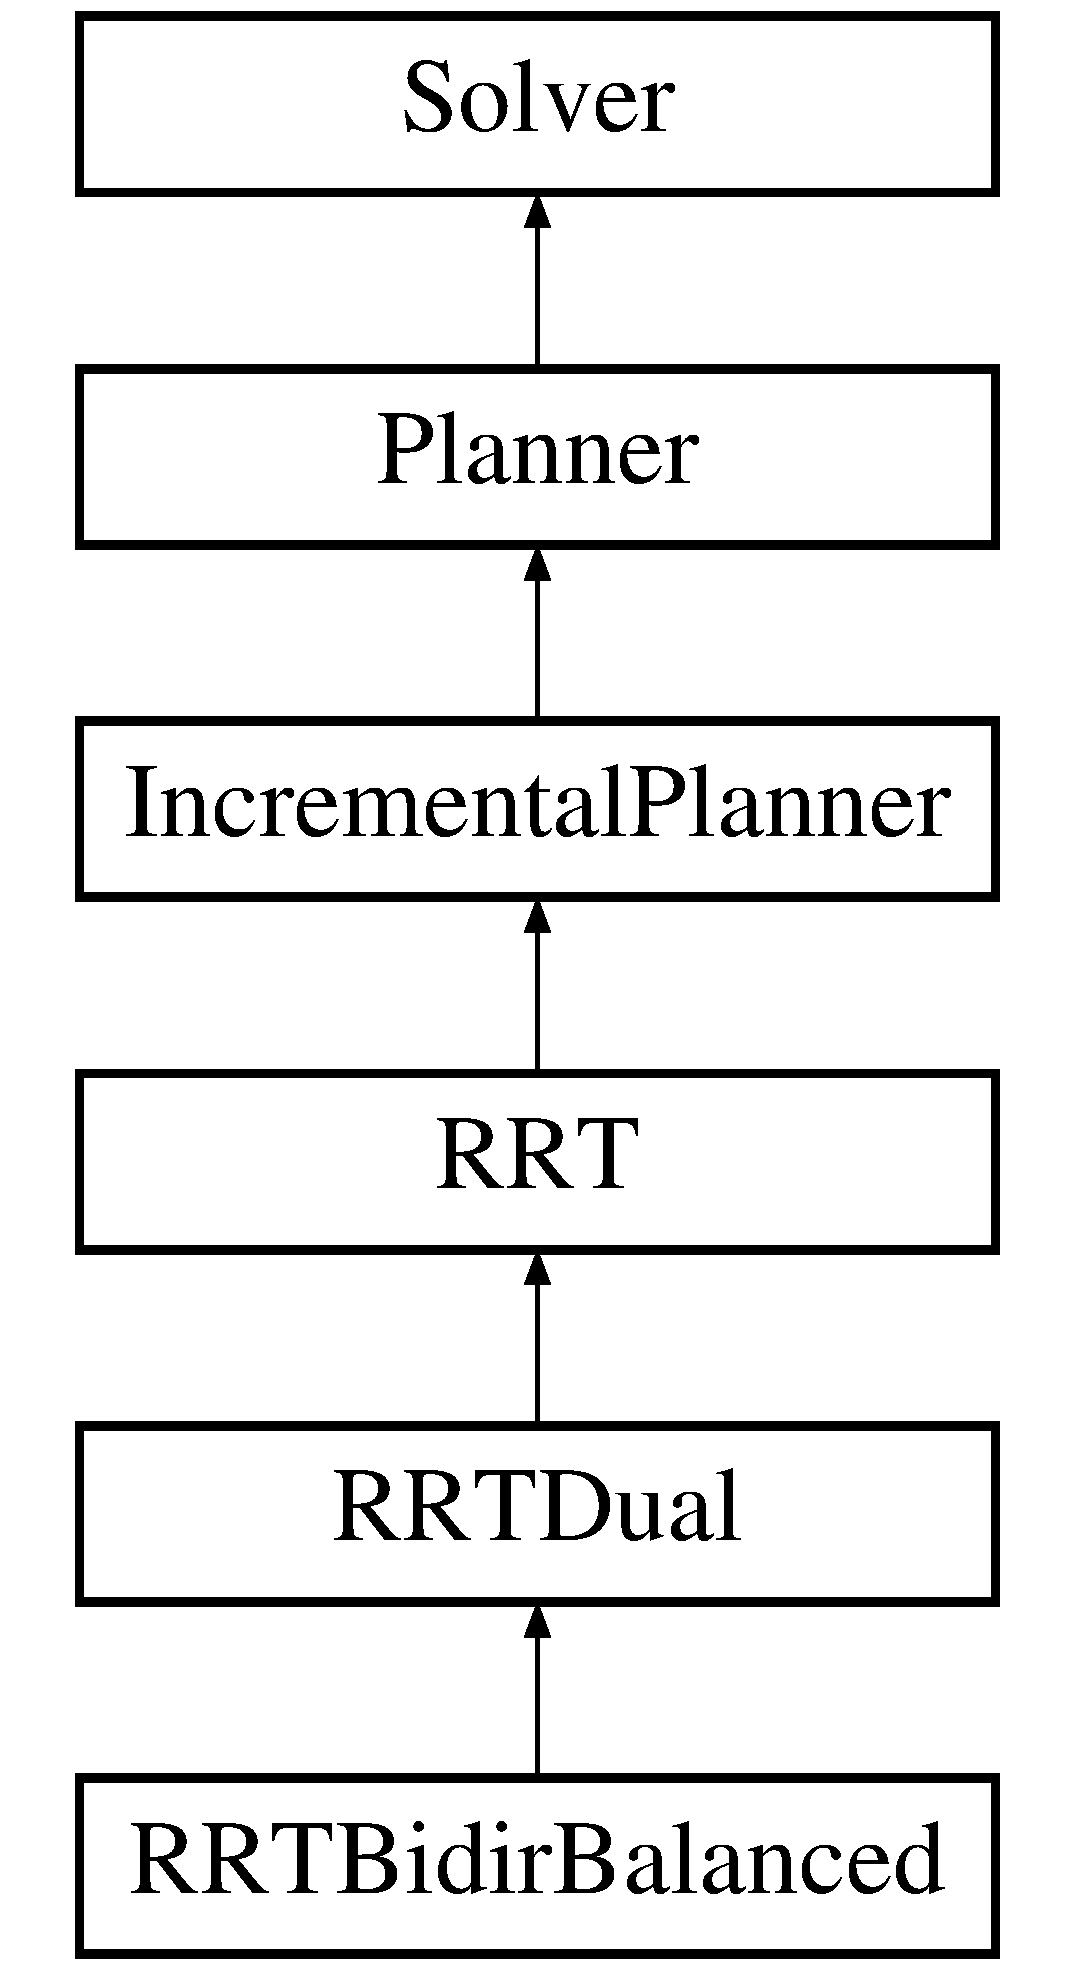
\includegraphics[height=6cm]{classRRTBidirBalanced}
\end{center}
\end{figure}
\subsection*{Public Methods}
\begin{CompactItemize}
\item 
{\bf RRTBidir\-Balanced} ({\bf Problem} $\ast$p)
\item 
virtual {\bf $\sim$RRTBidir\-Balanced} ()
\item 
virtual bool {\bf Plan} ()
\begin{CompactList}\small\item\em First planner to solve the alpha 1.0 puzzle Very fast for holonomic planning.\item\end{CompactList}\end{CompactItemize}


\subsection{Detailed Description}
Balanced Bidirectional {\bf RRTCon\-Con} {\rm (p.\,\pageref{classRRTConCon})} planner.

This planner behaves similar to {\bf RRTCon\-Con} {\rm (p.\,\pageref{classRRTConCon})}, except that a cardinality criteria is introduced to maintain relative balance between the number of nodes in each tree.

At each iteration, the tree with the fewest nodes is selected as the active tree. The planner attempts to add a new branch to the currently active tree using the Connect step.

Keeping the trees balanced has the dual effect of minimizing the overall number of nearest-neighbor calculations, and efficiently solving problems in which either of the initial or goal configurations is highly constrained relative to the other (as is often the case with assembly or disassembly planning).

This planner is able to consistently solve the original well-known alpha puzzle motion planning benchmark.

The planner is described in Kuffner, La\-Valle, Yang, 2002 



\subsection{Constructor \& Destructor Documentation}
\index{RRTBidirBalanced@{RRTBidir\-Balanced}!RRTBidirBalanced@{RRTBidirBalanced}}
\index{RRTBidirBalanced@{RRTBidirBalanced}!RRTBidirBalanced@{RRTBidir\-Balanced}}
\subsubsection{\setlength{\rightskip}{0pt plus 5cm}RRTBidir\-Balanced::RRTBidir\-Balanced ({\bf Problem} $\ast$ {\em p})}\label{classRRTBidirBalanced_a0}


\index{RRTBidirBalanced@{RRTBidir\-Balanced}!~RRTBidirBalanced@{$\sim$RRTBidirBalanced}}
\index{~RRTBidirBalanced@{$\sim$RRTBidirBalanced}!RRTBidirBalanced@{RRTBidir\-Balanced}}
\subsubsection{\setlength{\rightskip}{0pt plus 5cm}RRTBidir\-Balanced::$\sim$RRTBidir\-Balanced ()\hspace{0.3cm}{\tt  [inline, virtual]}}\label{classRRTBidirBalanced_a1}




\subsection{Member Function Documentation}
\index{RRTBidirBalanced@{RRTBidir\-Balanced}!Plan@{Plan}}
\index{Plan@{Plan}!RRTBidirBalanced@{RRTBidir\-Balanced}}
\subsubsection{\setlength{\rightskip}{0pt plus 5cm}bool RRTBidir\-Balanced::Plan ()\hspace{0.3cm}{\tt  [virtual]}}\label{classRRTBidirBalanced_a2}


First planner to solve the alpha 1.0 puzzle Very fast for holonomic planning.



Reimplemented from {\bf RRTDual} {\rm (p.\,\pageref{classRRTDual_a2})}.

The documentation for this class was generated from the following files:\begin{CompactItemize}
\item 
{\bf rrt.h}\item 
{\bf rrt.C}\end{CompactItemize}
